% GENERATED FROM typst/manual/sections/06_field_dynamics_applications.typ BY scripts/typ2tex.py (v1.0.0) — DO NOT EDIT.
% Edit canonical Typst under typst/ and regenerate with: python3 scripts/typ2tex.py --root . --outdir latex

\clearpage

\section{Field Dynamics Applications}\label{manual:field-dynamics-applications}

\paragraph{Calculation card.}
The coordinate examples use fixed exact tracks and integer comparators;
SPARC uses source radial rows and declared component proxies, with an
observation-only square-speed diagnostic. Tau retains carried score records,
and the orbital-retention path remains a required-input plan. Each subsection
keeps its scope, operator chain, output and falsifier. Source assumptions,
shared calibration and missing model uncertainty follow
\secref{manual:calculation-spine}; these evidence classes are distinct.

\aodnoteblock{Scope}{This section uses the main-note field dynamics calculus as an application layer. SPARC uses the square-speed coordinate $U=V^2$. The Tau ring fixture uses $S_{\tau}$ and missing-burden diagnostics. Each score coordinate is declared inside its own support class.}

\aodremark{Field-dynamics simulations are finite compressions of the A$\Omega$D ontology. A macroscopic field is simulated by declared clustering, finite boundary windows, support families, and value maps. Output residuals are read against the declared data support: boundary placement, density resolution, time-flow data, angular/radial momentum inputs, slosh windows, capacity seating, and sheddic-route declarations.}

A large field-dynamics system is handled by declared clustering. A cluster records a retained family of distinctions and relations over a boundary/window. The cluster records its support expression, construction trace or inherited trace, capacity rule, coupling family, and route status. The cluster is a finite calculation container recording a declared A$\Omega$D form.
A reduction declares its retained and discarded state, lineage and memory,
then tests the intended readout, error bound or future boundary response on
matched windows and interventions. Equal present summaries do not establish
future sufficiency; two histories with that summary and different next
responses refute it. No Markov closure follows from clustering alone.

\subsection{Data-support classes for manual simulations and comparisons}\label{manual:field-dynamics-data-support-classes}

The support rule in \secref{manual:scoped-errors-data-support} selects the comparison coordinate; it does not certify replay or physical validation. \tabref{tab:manual-data-support-classes} records the manual classes used by this release.

\begin{table}[H]
\centering
\caption{Data-support classes for manual simulations and comparisons.}
\label{tab:manual-data-support-classes}
{\footnotesize
\begin{tabular}{>{\raggedright\arraybackslash}p{0.070\linewidth}>{\raggedright\arraybackslash}p{0.170\linewidth}>{\raggedright\arraybackslash}p{0.270\linewidth}>{\raggedright\arraybackslash}p{0.220\linewidth}>{\raggedright\arraybackslash}p{0.120\linewidth}}
\toprule
Class & Name & Declared distinctions & Relations induced & Residual \\
\midrule
D0 & exact internal fixture & exact integer gates, channels, comparator bins & internal returned-current relations & $\delta_3$ tally \\
O0 & observable-map fixture & observable-map value and measured-sector target & external comparison map & target residual \\
G0 & radial shell projection & galaxy, radial bin, radius, speed, radial gas/disk/bulge support & radial shell field-dynamics relations & $U$ residuals \\
G1 & radial-medium projection & G0 plus radial density/current proxy fields & radial medium-support relations & $U$ + proxy \\
G2 & 3D shell field-dynamics retention & radial, angular, vertical cells; density, velocity, current, background support & local/inter/core/long/bg/J range SADAR & retention / field \\
G3 & time-resolved tracer-current simulation & G2 plus tracer positions/velocities through time windows & slosh, hinge shift, chiral flip, partial coupling & path / phase \\
L0 & exact lensing toy fixture & exact gates and comparator tallies & field-ring $\delta_3$ relations & $\delta_3$ tally \\
L1 & radial lens-medium diagnostic & radial medium proxies without image targets & medium-class relations & medium tallies \\
L2 & target-acquisition lane & image-count, Einstein-radius, image-position, or shear targets & target-side quarantine & acquisition \\
L3 & full lensing input package & declared medium fields, radiation-current gates, and target side & prediction before target join; target scoring after freeze & lens residuals \\
\bottomrule
\end{tabular}
}
\end{table}

\aodremark{This table records which distinctions are instantiated by a manual calculation. Projection and marginalization maps record comparison coordinates and uncertainty.}

\subsection{Data-support and uncertainty budget}\label{manual:field-dynamics-data-support-budget}

A field-dynamics diagnostic records its data-support and uncertainty budget before residuals are interpreted. The budget records the declared distinction family, support class, uncertainty component, and report target.

\begin{table}[H]
\centering
\caption{Field dynamics data-support classes.}
\label{tab:field-dynamics-data-support-budget-a}
{\footnotesize
\begin{tabular}{>{\raggedright\arraybackslash}p{0.160\linewidth}>{\raggedright\arraybackslash}p{0.080\linewidth}>{\raggedright\arraybackslash}p{0.420\linewidth}>{\raggedright\arraybackslash}p{0.260\linewidth}}
\toprule
Distinction family & Symbol & Declared data support & Support class \\
\midrule
Density & $\epsilon_{\rho}$ & $\rho(R,z,\theta,t)$ or radial proxy & 3D / 2D / radial / proxy \\
Velocity & $\epsilon_v$ & $v(R,z,\theta,t)$ or radial speed & vector / radial / proxy \\
Time window & $\epsilon_{\omega}$ & cadence and duration & measured / declared / proxy \\
Boundary & $\epsilon_{\partial}$ & $\partial_TR_c(t)$ & 3D / radial / proxy \\
Capacity & $\epsilon_C$ & $C^{\mathrm{cap}}$ & typed / scalar / inherited / proxy \\
Coupling & $\epsilon_E$ & $E^{\mathfrak{S}}(B)$ & full / radial / proxy / ablation cut \\
Sheddic route & $\epsilon_X$ & $\operatorname{SheddicPath}$ & declared / inferred \\
External map & $\epsilon_K$ & $K_{\mathrm{ext}}$ or $\lambda$ & frozen / calibrated \\
\bottomrule
\end{tabular}
}
\end{table}

\begin{table}[H]
\centering
\caption{Field dynamics uncertainty and report targets.}
\label{tab:field-dynamics-data-support-budget-b}
{\footnotesize
\begin{tabular}{>{\raggedright\arraybackslash}p{0.160\linewidth}>{\raggedright\arraybackslash}p{0.080\linewidth}>{\raggedright\arraybackslash}p{0.320\linewidth}>{\raggedright\arraybackslash}p{0.360\linewidth}}
\toprule
Distinction family & Symbol & Uncertainty & Report target \\
\midrule
Density & $\epsilon_{\rho}$ & $\sigma_{\rho}$ when declared & field or $U$ \\
Velocity & $\epsilon_v$ & $\sigma_v$ & current, path, or $U$ \\
Time window & $\epsilon_{\omega}$ & $\sigma_{\omega}$ & slosh / retention / path \\
Boundary & $\epsilon_{\partial}$ & $\sigma_{\partial}$ & boundary audits \\
Capacity & $\epsilon_C$ & $\sigma_C$ & retention / seating \\
Coupling & $\epsilon_E$ & $\sigma_E$ & retention / projection \\
Sheddic route & $\epsilon_X$ & $\sigma_X$ & route / slosh \\
External map & $\epsilon_K$ & $\sigma_{\mathrm{map}}$ & external comparison \\
\bottomrule
\end{tabular}
}
\end{table}

\aodremark{A scored diagnostic is interpreted within its declared support class. Projection and marginalization comparisons report their uncertainty records.}

\paragraph{Ablation cut.}
An ablation cut is a declared data-support cut with one distinction family intentionally omitted or marginalized. It records projection or marginalization residuals against a comparison support class. The evaluated A$\Omega$D form remains the declared form for that record.

\subsection{Scoped error forms by data-support class}\label{manual:field-dynamics-scoped-error-forms}

For a G0 radial shell projection, the score coordinate remains square speed:

\[
U^{\mathrm{obs}}_{g,j}=(V^{\mathrm{obs}}_{g,j})^2,\qquad\Delta U_{g,j}=U^{A\Omega}_{g,j}-U^{\mathrm{obs}}_{g,j}.
\]

When observation, projection and input contributions form a justified joint
moment model with zero cross-covariances, their residual variance reduces to

\[
\sigma^2_{\mathrm{total},g,j}=\sigma^2_{\mathrm{obs},g,j}+\sigma^2_{\mathrm{proj},g,j}+\sigma^2_{\mathrm{input},g,j},\qquad z^U_{g,j}=\frac{U^{A\Omega}_{g,j}-U^{\mathrm{obs}}_{g,j}}{\sigma_{\mathrm{total},g,j}}.
\]

For a G1 radial-medium projection, proxy-support residuals may be recorded as

\[
\epsilon_{\rho,j}=\rho^{A\Omega}_j-\rho^{\mathrm{proxy}}_j,\qquad\epsilon_{J,j}=J^{A\Omega}_j-J^{\mathrm{proxy}}_j.
\]

For a G2 three-dimensional field-dynamics retention fixture, exact retention tallies and field residuals may be recorded as

\[
\Delta^{\mathbb{Z}}_k=T_k-O_k,\qquad\delta_{3,k}=(s^{(3)}_k,m_k),
\]

\[
\epsilon_{\rho}(c)=\rho^{A\Omega}_c-\rho^{\mathrm{obs}}_c,\qquad J^{\mathrm{obs}}_c=\rho^{\mathrm{obs}}_cv^{\mathrm{obs}}_c,\qquad\epsilon_J(c)=J^{A\Omega}_c-J^{\mathrm{obs}}_c.
\]

For vector targets, the fixture declares $\varepsilon\ge0$ with the units of $\|J^{A\Omega}_c\|\,\|J^{\mathrm{obs}}_c\|$ and a positive denominator. The dimensionless regularized alignment score is

\[
c_{\varepsilon,c}=\frac{J^{A\Omega}_c\cdot J^{\mathrm{obs}}_c}{\|J^{A\Omega}_c\|\,\|J^{\mathrm{obs}}_c\|+\varepsilon}.
\]

For a G3 time-resolved tracer-current fixture, path and velocity residuals such as $\epsilon_x$ and $\epsilon_v$ are declared against path-coordinate targets. RMSE reports are used only when the fixture declares metric units and path-coordinate targets.

\subsection{Two-dimensional slice / three-dimensional field toy}\label{manual:2d-3d-slice-toy}

This toy records how data-support scope changes the reported value when a three-dimensional field is represented by a two-dimensional slice or when the boundary is placed improperly. It is a manual diagnostic container that records declared comparison values.

Let $B_{3D}$ be the declared three-dimensional boundary/window and let $B_{2D}$ be the slice boundary obtained by suppressing the vertical/time-flow input. Let $B_{\mathrm{bad}}$ be an intentionally improper setup boundary. The same calculation is evaluated three ways:

\[
U^{3D}_{\AO}=\mathsf{Q}^U_{\mathrm{ext}}(D^{\mathrm{BF}}(B_{3D})),\qquad U^{2D}_{\AO}=\mathsf{Q}^U_{\mathrm{ext}}(D^{\mathrm{BF}}(B_{2D})),\qquad U^{\mathrm{bad}}_{\AO}=\mathsf{Q}^U_{\mathrm{ext}}(D^{\mathrm{BF}}(B_{\mathrm{bad}})).
\]

The scoped diagnostics are

\[
\Delta U_{2D\to3D}=U^{2D}_{\AO}-U^{3D}_{\AO},\qquad\Delta U_{\partial}=U^{\mathrm{bad}}_{\AO}-U^{3D}_{\AO}.
\]

For exact internal bins, the same comparison may be recorded by

\[
\Delta_k^{\mathbb{Z}}=T_k^{\mathrm{bad}}-T_k^{3D},\qquad\delta_{3,k}(T^{\mathrm{bad}},T^{3D})=(s_k^{(3)},m_k).
\]

\begin{table}[H]
\centering
\caption{Toy data-support cases.}
\label{tab:toy-data-support-cases}
{\footnotesize
\begin{tabular}{>{\raggedright\arraybackslash}p{0.180\linewidth}>{\raggedright\arraybackslash}p{0.220\linewidth}>{\raggedright\arraybackslash}p{0.240\linewidth}>{\raggedright\arraybackslash}p{0.200\linewidth}}
\toprule
Case & Boundary / data & Diagnostic & Interpretation \\
\midrule
3D declared field & $B_{3D}$, $\rho(R,z,\theta,t)$, velocity and window data & baseline value $U^{3D}_{\AO}$ or $T^{3D}$ & retained support reference \\
2D slice & $B_{2D}$, vertical/time-flow suppressed & $\Delta U_{2D\to3D}$ & slice projection residual \\
Improper boundary & $B_{\mathrm{bad}}$, wrong boundary/capacity/route & $\Delta U_{\partial}$ or $\delta_3(T^{\mathrm{bad}},T^{3D})$ & boundary-support residual \\
\bottomrule
\end{tabular}
}
\end{table}

\aodremark{This toy shows why field dynamics must record boundary declarations and data-support class. A two-dimensional slice and a three-dimensional field are different declared support classes; residuals between them are projection or boundary-support residuals before any external target comparison is interpreted.}

\subsection{3D Brownian phase-cycle \texorpdfstring{$\delta_3$}{delta3} fixture}\label{manual:brownian-phase-delta3-fixture}

\aodnoteblock{Data-support class}{This Brownian / tracer-motion fixture is a G3 time-resolved tracer-current fixture when the track declares time-ordered three-dimensional positions. A two-dimensional microscopy slice records its projection map or ablation cut.}

This fixture uses integerized three-dimensional trajectory data. A bacterium or tracer track is binned into $\mathbb{Z}^3$; lagged displacements produce the active integer squared displacement

\[
Q_i^{(n)}=(a_i^{(n)})^2+(b_i^{(n)})^2+(c_i^{(n)})^2\in\mathbb{Z}_{\ge0}.
\]

A declared mass/size adapter may supply a candidate monon-beat scale $\beta_a$; the fixed fixture does not instantiate measured acquisition. The trajectory is tested by displacement-bin counts, phase-cycle counts $Q_i^{(n)}\bmod\beta_a$, octant direction counts, integer ratios, and exact $\delta_3$ residuals. The full 3D coordinate phase-cycle specification is given in \appref{manual:app:coordinate-phase-cycle-delta3}.

The exact fixture path is

\[
z_i\in\mathbb{Z}^3\to\Delta z_i^{(n)}\to Q_i^{(n)}\to\theta_i^{(n)}\to O_{\theta}^{(n)}\to\delta_3.
\]

The retained trace path is

\[
\Delta z_i^{(n)}\to HT(h_i;B_{\mathrm{mot}})\to RD_{h_i}\to RCD_{h_i}\to\rho^D_{\omega,h_i}\to\SADARop_B.
\]

Continuous summaries belong after the exact fixture as presentation or external maps.

\aodnoteblock{Source artifacts}{The source package includes the Brownian application script under \texttt{manual/scripts} and the Brownian CSV rows under \texttt{manual/data/brownian}:

\begin{gather*}
\mathtt{aod\_brownian\_3d\_phase\_delta3.py},\quad\mathtt{displacement\_q\_counts.csv},\quad\mathtt{phase\_cycle\_delta3.csv},\\\mathtt{octant\_delta3.csv},\quad\mathtt{integer\_motion\_ratios.csv}.
\end{gather*}

These Brownian application artifacts are aliases of the generic 3D coordinate phase-cycle fixture specified in \appref{manual:app:coordinate-phase-cycle-delta3}.}

\aodremark{Active coordinate: integerized three-dimensional displacement and phase-cycle count data,

\[
z_i\in\mathbb{Z}^3\to\Delta z_i^{(n)}\to Q_i^{(n)}\to\theta_i^{(n)}\to O_{\theta}^{(n)}\to\delta_3.
\]

Continuous Brownian and diffusion-coefficient summaries are downstream presentation maps.}

\subsubsection{Run-tumble tracer-current fixture}\label{manual:run-tumble-tracer-current-fixture}

\aodnoteblock{Data-support class}{This run-tumble record is a G3 time-resolved tracer-current fixture. Its exact integer tallies are recorded as D0-style internal fixture audit coordinates when a comparator is declared.}

This fixture records a finite D.E.C. trace over four declared Hamming--1 edge slots, stores the selected signed edge steps as a four-channel accumulated trace, and projects that retained trace into a declared three-dimensional coordinate map before phase-cycle, octant, and $\delta_3$ summaries are formed. Declare

\[
B_{\mathrm{RT}}=(\partial_TF_{\mathrm{RT}},\omega_{20}),\qquad\omega_{20}=\{0,1,\dots,20\},\qquad E_4=\{e_1,e_2,e_3,e_4\}.
\]

The accumulated trace is

\[
h_t\in\mathbb{Z}^4,\qquad h_0=(0,0,0,0),
\]

with update

\[
h_t=h_{t-1}+\sigma_t\mathbf{e}_{j_t},\qquad j_t\in\{1,2,3,4\},\qquad\sigma_t\in\{-1,+1\}.
\]

The run/tumble mode is

\[
m_t\in\{\mathrm{run},\mathrm{tumble}\}.
\]

Run retains the active channel over the declared short window. Tumble reseats the active channel by the declared isotropic successor rule. The generated trace includes the initial row $t=0$ with $h_0=(0,0,0,0)$; run/tumble mode is assigned for the update rows $t\ge1$. The projection map is declared before any three-dimensional quantity is reported:

\[
\pi_3:\mathbb{Z}^4\to\mathbb{Z}^3,\qquad z_t=\pi_3(h_t).
\]

For the released fixture,

\[
\pi_3(h_1,h_2,h_3,h_4)=(h_1,h_2,h_3).
\]

The fourth trace channel remains part of the $Q^2_4$ audit even when it is not carried by the released $\pi_3$ projection. The active three-dimensional squared-displacement audit quantity is

\[
Q^2_{3D}(t)=x_t^2+y_t^2+z_t^2,\qquad\pi_3(h_t)=(x_t,y_t,z_t).
\]

The four-channel audit displacement is

\[
Q^2_4(t)=h_{1,t}^2+h_{2,t}^2+h_{3,t}^2+h_{4,t}^2.
\]

Here $Q^2_{3D}$ and $Q^2_4$ are local squared-displacement audit quantities, not $Q^D$ pending-overhang notation. The fixture records $Q^2_{3D}$, $Q^2_4$, phase residues $Q^2_{3D}\bmod\beta_a$, octant counts, integer ratios, and exact $\delta_3$ residuals. Continuous Brownian, diffusion, and stochastic-calculus summaries are downstream presentation maps.

\begin{table}[H]
\centering
\caption{Run-tumble tracer-current declaration.}
\label{tab:run-tumble-tracer-declaration}
{\footnotesize
\begin{tabularx}{\linewidth}{>{\raggedright\arraybackslash}p{0.240\linewidth}>{\raggedright\arraybackslash}X}
\toprule
Item & Declaration \\
\midrule
support & four Hamming--1 edge slots $E_4=\{e_1,e_2,e_3,e_4\}$ \\
accumulated trace & $h_t\in\mathbb{Z}^4$ \\
projection & $\pi_3:\mathbb{Z}^4\to\mathbb{Z}^3$ \\
projected coordinate & $z_t=\pi_3(h_t)\in\mathbb{Z}^3$ \\
mode & $m_t\in\{\mathrm{run},\mathrm{tumble}\}$ \\
run rule & retain selected channel over declared short window \\
tumble rule & reseat selected channel by isotropic successor rule \\
3D displacement & $Q^2_{3D}(t)=x_t^2+y_t^2+z_t^2$ \\
four-channel audit & $Q^2_4(t)=\sum_{r=1}^4h_{r,t}^2$ \\
reports & phase counts, octant counts, integer ratios, $\delta_3$ \\
\bottomrule
\end{tabularx}
}
\end{table}

% GENERATED FROM typst/manual/tables/run_tumble_trace_table.typ BY scripts/typ2tex.py (v1.0.0) — DO NOT EDIT.
% Edit canonical Typst under typst/ and regenerate with: python3 scripts/typ2tex.py --root . --outdir latex

\begin{table}[H]
\centering
\caption{Run-tumble tracer-current 20-tick exact trace.}
\label{tab:run-tumble-tracer-current-20tick}
{\footnotesize
\begin{tabular}{rllrllrrrr}
\toprule
$t$ & mode & edge & $\sigma$ & $h_t$ & $\pi_3(h_t)$ & $Q^2_{3D}$ & $Q^2_4$ & $\theta$ & oct. \\
\midrule
0 & init & - & -- & \texttt{(0,0,0,0)} & \texttt{(0,0,0)} & 0 & 0 & 0 & 0 \\
1 & run & e1 & +1 & \texttt{(1,0,0,0)} & \texttt{(1,0,0)} & 1 & 1 & 1 & 0 \\
2 & run & e1 & +1 & \texttt{(2,0,0,0)} & \texttt{(2,0,0)} & 4 & 4 & 4 & 0 \\
3 & tumble & e2 & +1 & \texttt{(2,1,0,0)} & \texttt{(2,1,0)} & 5 & 5 & 0 & 0 \\
4 & run & e2 & +1 & \texttt{(2,2,0,0)} & \texttt{(2,2,0)} & 8 & 8 & 3 & 0 \\
5 & tumble & e3 & -1 & \texttt{(2,2,-1,0)} & \texttt{(2,2,-1)} & 9 & 9 & 4 & 4 \\
6 & run & e3 & -1 & \texttt{(2,2,-2,0)} & \texttt{(2,2,-2)} & 12 & 12 & 2 & 4 \\
7 & tumble & e4 & +1 & \texttt{(2,2,-2,1)} & \texttt{(2,2,-2)} & 12 & 13 & 2 & 4 \\
8 & run & e4 & +1 & \texttt{(2,2,-2,2)} & \texttt{(2,2,-2)} & 12 & 16 & 2 & 4 \\
9 & tumble & e1 & -1 & \texttt{(1,2,-2,2)} & \texttt{(1,2,-2)} & 9 & 13 & 4 & 4 \\
10 & run & e1 & -1 & \texttt{(0,2,-2,2)} & \texttt{(0,2,-2)} & 8 & 12 & 3 & 4 \\
11 & tumble & e2 & -1 & \texttt{(0,1,-2,2)} & \texttt{(0,1,-2)} & 5 & 9 & 0 & 4 \\
12 & run & e2 & -1 & \texttt{(0,0,-2,2)} & \texttt{(0,0,-2)} & 4 & 8 & 4 & 4 \\
13 & tumble & e3 & +1 & \texttt{(0,0,-1,2)} & \texttt{(0,0,-1)} & 1 & 5 & 1 & 4 \\
14 & run & e3 & +1 & \texttt{(0,0,0,2)} & \texttt{(0,0,0)} & 0 & 4 & 0 & 0 \\
15 & tumble & e4 & -1 & \texttt{(0,0,0,1)} & \texttt{(0,0,0)} & 0 & 1 & 0 & 0 \\
16 & run & e4 & -1 & \texttt{(0,0,0,0)} & \texttt{(0,0,0)} & 0 & 0 & 0 & 0 \\
17 & tumble & e1 & +1 & \texttt{(1,0,0,0)} & \texttt{(1,0,0)} & 1 & 1 & 1 & 0 \\
18 & run & e1 & +1 & \texttt{(2,0,0,0)} & \texttt{(2,0,0)} & 4 & 4 & 4 & 0 \\
19 & tumble & e2 & +1 & \texttt{(2,1,0,0)} & \texttt{(2,1,0)} & 5 & 5 & 0 & 0 \\
20 & run & e2 & +1 & \texttt{(2,2,0,0)} & \texttt{(2,2,0)} & 8 & 8 & 3 & 0 \\
\bottomrule
\end{tabular}
}
\end{table}


\begin{figure}[H]
\centering
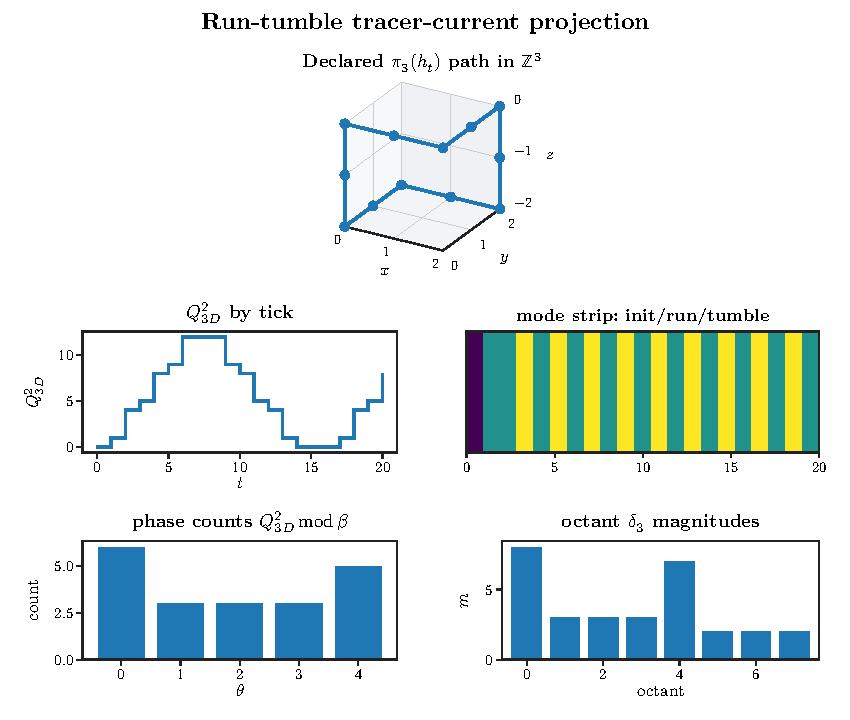
\includegraphics[width=0.92\linewidth,height=0.78\textheight,keepaspectratio]{figures/generated/run-tumble-trace-3d-projection.pdf}
\caption{Run-tumble tracer-current projection. The plotted path is the declared $\mathbb{Z}^3$ projection of the retained $\mathbb{Z}^4$ accumulated trace. The finite $Q_4$ support remains the Hamming--1 edge-slot support.}
\label{fig:run-tumble-tracer-current-projection}
\end{figure}

\aodnoteblock{Source artifacts}{The source package includes the deterministic run-tumble generator \texttt{manual/scripts/aod\_run\_tumble\_3d\_trace.py}, the generated trace table, the run-tumble CSV outputs under \texttt{manual/data/run\_tumble}, and the projection figure under \texttt{manual/figures}.}

\subsection{SPARC square-speed diagnostic}\label{manual:sparc-square-speed-diagnostic}

The SPARC five-galaxy square-speed score is the current G0 radial shell field-dynamics diagnostic lane. This record uses SPARC radial rotation-curve rows, scores the coordinate $U=V^2$, forms $\sigma_U=2V^{\mathrm{obs}}\sigma_V$ from the declared data uncertainty, and records $\Delta U=U_{\AO}-U^{\mathrm{obs}}$ inside the G0 support class.
The SPARC benchmark supplies declared galaxy records

\[
\mathcal{D}_{\mathrm{SPARC}}=\{G_i,r_{ij},V^{\mathrm{obs}}_{ij},\sigma_{V,ij},V^{\mathrm{gas}}_{ij},V^{\mathrm{disk}}_{ij},V^{\mathrm{bulge}}_{ij},\dots\}.
\]

The score coordinate is square speed:

\[
U^{\mathrm{obs}}_{g,j}=(V^{\mathrm{obs}}_{g,j})^2,\qquad\sigma_{U,g,j}=2V^{\mathrm{obs}}_{g,j}\sigma_{V,g,j}.
\]

The displayed $\sigma_U=2V^{\mathrm{obs}}\sigma_V$ is first-order
propagation about a positive measured speed, appropriate only where its
nonlinear remainder is negligible for the claimed precision. It is not an
exact square-map uncertainty. The present scores use this observation-only
diagnostic; input-proxy, distance, inclination, map and shared-source
contributions are not thereby zero. Exact finite laws or justified bounds
use the M3 routes in \secref{manual:scoped-errors-data-support}. The declared score target is $U^{\mathrm{obs}}_{g,j}$, and benchmark input columns remain input data until the report map is evaluated. This G0 diagnostic uses nonnegative component proxies

\[
U^k_{g,j}:=(V^k_{g,j})^2,\qquad k\in\{\mathrm{gas},\mathrm{disk},\mathrm{bulge}\}.
\]

SPARC's signed gas contribution is $V^{\mathrm{gas}}|V^{\mathrm{gas}}|$. The retained proxy $U^{\mathrm{gas}}=(V^{\mathrm{gas}})^2$ preserves its magnitude and removes the contribution sign for negative source entries.

\[
U^{\mathrm{bar}}_{g,j}=U^{\mathrm{gas}}_{g,j}+\Upsilon_dU^{\mathrm{disk}}_{g,j}+\Upsilon_bU^{\mathrm{bulge}}_{g,j}.
\]

The release constants are frozen before residuals are computed:

\[
\Upsilon_d=\frac{1}{2},\qquad\Upsilon_b=\frac{7}{10},\qquad K^U_{\mathrm{ext}}=8,\qquad J_{\mathrm{norm}}=1.
\]

The retained-window ratio uses the scalar duration accessor, not the RCD coupling object:

\[
\lambda^{\mathrm{ret}}_{g,j}:=\frac{\rho^D_{\omega,g,j}}{\rho^D_{g,j}}.
\]

The released field-dynamics support term is

\[
D^{\mathrm{BF}}_{g,j}=C_{\mathrm{cap},g,j}\lambda^{\mathrm{ret}}_{g,j}(1+\frac{\mathrm{density}_{g,j}}{16})(1+\frac{\mathrm{gas/star}_{g,j}}{16})(1+\frac{\mathrm{bobbing}_{g,j}}{64})J_{\mathrm{norm}}.
\]

In the five-galaxy G0/G1 diagnostic lane, the declared primary projection map uses

\[
C_{\mathrm{cap},g,j}=r_{g,j}(|V^{\mathrm{gas}}_{g,j}|+|V^{\mathrm{disk}}_{g,j}|+|V^{\mathrm{bulge}}_{g,j}|),\quad\lambda^{\mathrm{ret}}_{g,j}=1,\quad\mathrm{density}_{g,j}=\mathrm{gas/star}_{g,j}=\mathrm{bobbing}_{g,j}=0.
\]

This neutral modifier convention belongs to the declared radial projection map. G1/G2/G3 packages carry angular, vertical, or time-flow fields through declared source or proxy rows.
The external square-speed map is

\[
U_{g,j,\AO}=U^{\mathrm{bar}}_{g,j}+K^U_{\mathrm{ext}}D^{\mathrm{BF}}_{g,j}.
\]

Here $K^U_{\mathrm{ext}}$ is a quarantined external map coefficient frozen before scoring and used only by the external-comparison layer.

\[
\operatorname{scope}(K^U_{\mathrm{ext}})=\text{external square-speed value map},\qquad[K^U_{\mathrm{ext}}]=\frac{(\mathrm{km/s})^2}{\mathrm{kpc}\cdot(\mathrm{km/s})}=\frac{\mathrm{km/s}}{\mathrm{kpc}}.
\]

\aodliteraturenote{SPARC benchmark: SPARC database~\cite{sparc-database}, Lelli et al.~\cite{lelli-sparc-2016}.}

\aodnoteblock{Data-support class}{The SPARC five-galaxy lane instantiates a G0 radial shell data-support class. G0 active input fields are $G_i,r_{ij},V^{\mathrm{obs}}_{ij},\sigma_{V,ij},V^{\mathrm{gas}}_{ij},V^{\mathrm{disk}}_{ij},V^{\mathrm{bulge}}_{ij}$. The report coordinate is $U=(V^{\mathrm{obs}})^2$, $\sigma_U=2V^{\mathrm{obs}}\sigma_V$, and $\Delta U=U_{\AO}-U^{\mathrm{obs}}$. G1/G2/G3 packages carry angular, vertical, or time-flow fields through declared source or proxy rows.}

\subsection{SPARC five-galaxy scored records}\label{manual:sparc-five-galaxy-scored}

The five scored records are

\[
\{\mathrm{NGC2403},\mathrm{NGC3198},\mathrm{NGC6503},\mathrm{NGC2841},\mathrm{DDO154}\}.
\]

Data files, scored outputs, and the regeneration script are included in the source package:

\begin{align*}
 & \mathtt{manual/data/sparc},\\ & \mathtt{manual/data/derived/sparc\_five\_galaxy\_per\_bin.csv},\\ & \mathtt{manual/data/derived/sparc\_five\_galaxy\_per\_galaxy.csv},\\ & \mathtt{manual/scripts/score\_sparc\_field\_dynamics.py}.
\end{align*}

\aodremark{The SPARC five-galaxy scored records are generated from the included rotation-curve files and the frozen declaration constants listed in this section.}

\[
\Delta U_{g,j}=U_{g,j,\AO}-U^{\mathrm{obs}}_{g,j},\qquad z^U_{g,j}=\frac{\Delta U_{g,j}}{\sigma_{U,g,j}}.
\]

\[
\chi^2_{U,g}=\sum_j(z^U_{g,j})^2,\quad MAE_{U,g}=\frac{1}{N_g}\sum_j|\Delta U_{g,j}|,\quad MSE_{U,g}=\frac{1}{N_g}\sum_j(\Delta U_{g,j})^2.
\]

\[
MAPE_{U,g}=\frac{100}{N_g}\sum_j|\frac{\Delta U_{g,j}}{U^{\mathrm{obs}}_{g,j}}|,\qquad U^{\mathrm{obs}}_{g,j}>0.
\]

Bins are excluded only by a predeclared data-quality rule or by a predeclared denominator floor. Across all $209$ positive-$U^{\mathrm{obs}}$ radial bins of the five-galaxy sample, the reference engine (\texttt{manual/data/boundary\_sadar/sparc\_pooled\_primary\_exact.csv}, vector \texttt{SD-008}) evaluates the exact rational pooled primary score $MAPE_U=64.70291920\%$ ($1523$-digit numerator over $1521$-digit denominator), distinct from the carried control $66.1613\%$ in \texttt{sparc\_declaration\_controls.csv}.

% GENERATED FROM typst/manual/tables/sparc_summary_table.typ BY scripts/typ2tex.py (v1.0.0) — DO NOT EDIT.
% Edit canonical Typst under typst/ and regenerate with: python3 scripts/typ2tex.py --root . --outdir latex

\begin{table}[H]
\centering
\caption{SPARC five-galaxy scored records. Data-support class is G0 for this radial shell projection lane; the uncertainty policy is observation-only in this release.}
\label{tab:manual-sparc-five-galaxy-scores}
{\footnotesize
\begin{tabular}{lccrrrrr}
\toprule
$G$ & Class & $\sigma$ policy & $N$ & $\chi^2_U$ & $MAE_U$ & $MSE_U$ & $MAPE_U$ [\%] \\
\midrule
DDO154 & G0 & obs-only & 12 & 10893.83 & 697.2 & 602049.7 & 41.42 \\
NGC2403 & G0 & obs-only & 73 & 22038.64 & 2486.2 & 7212253.2 & 23.31 \\
NGC2841 & G0 & obs-only & 50 & 3235.74 & 23910.7 & 674670051.2 & 26.47 \\
NGC3198 & G0 & obs-only & 43 & 6352.96 & 5478.2 & 62935093.1 & 37.51 \\
NGC6503 & G0 & obs-only & 31 & 718.93 & 1697.4 & 3689898.7 & 13.50 \\
\bottomrule
\end{tabular}
}
\end{table}


\begin{figure}[H]
\centering
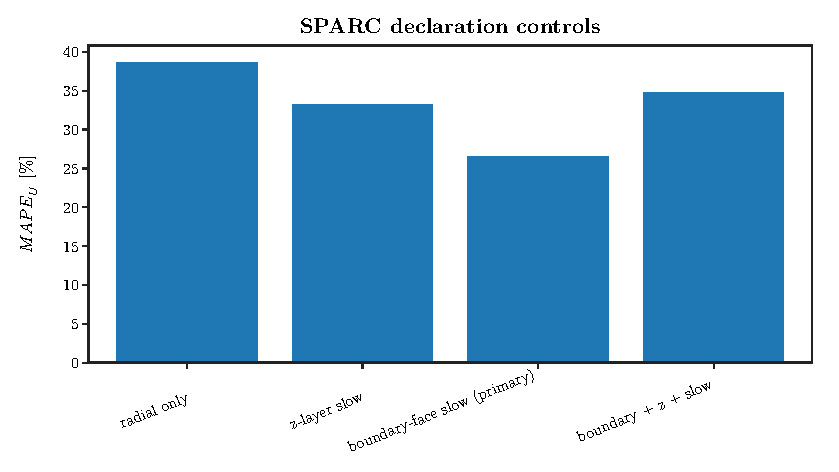
\includegraphics[width=0.92\linewidth,height=0.78\textheight,keepaspectratio]{figures/generated/sparc-declaration-controls.pdf}
\caption{SPARC carried declaration-control scores. The four values in \texttt{sparc\_declaration\_controls.csv} are frozen comparison records; their variant recipes and aggregation rule are not supplied. Primary per-bin and per-galaxy scores are computed separately by the declared map.}
\label{fig:manual-sparc-controls}
\end{figure}

\begin{figure}[H]
\centering
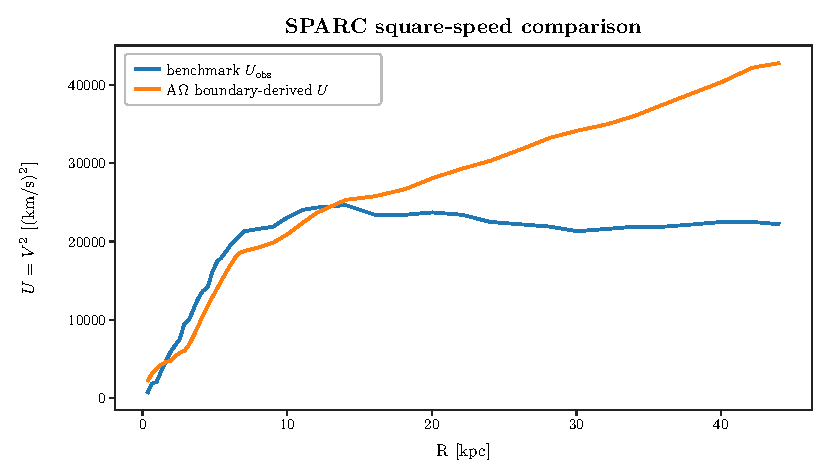
\includegraphics[width=0.92\linewidth,height=0.78\textheight,keepaspectratio]{figures/generated/sparc-square-speed-comparison.pdf}
\caption{SPARC square-speed comparison for the NGC3198 display record. The scored coordinate is $U=V^2$.}
\label{fig:manual-sparc-square-speed-comparison}
\end{figure}

\begin{figure}[H]
\centering
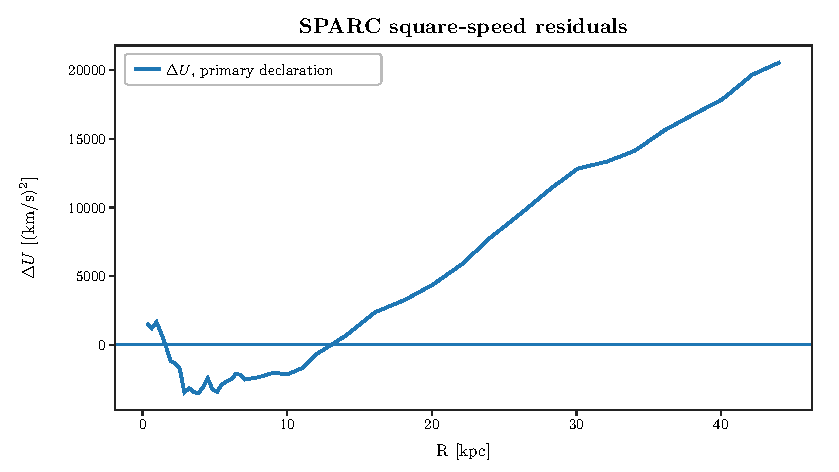
\includegraphics[width=0.92\linewidth,height=0.78\textheight,keepaspectratio]{figures/generated/sparc-square-speed-residuals.pdf}
\caption{SPARC square-speed residuals for the NGC3198 display record. The residual is $\Delta U=U_{\AO}-U_{\mathrm{obs}}$.}
\label{fig:manual-sparc-residuals}
\end{figure}

\begin{figure}[H]
\centering
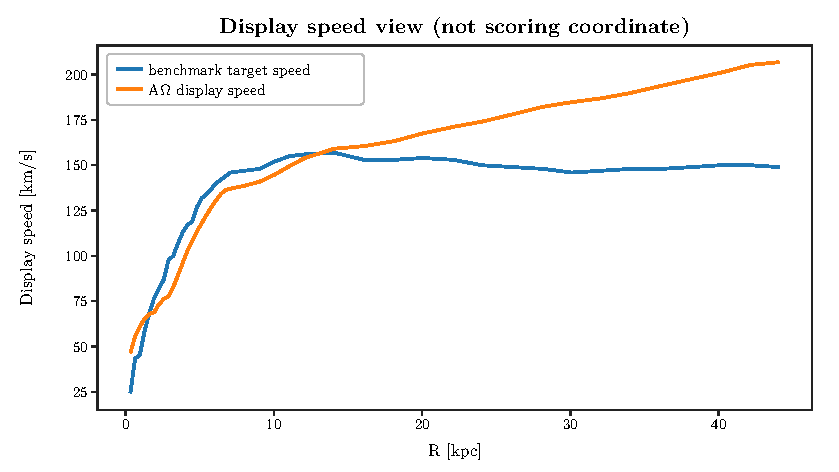
\includegraphics[width=0.92\linewidth,height=0.78\textheight,keepaspectratio]{figures/generated/sparc-display-speed-view.pdf}
\caption{Display speed view. This presentation view uses $V_{\mathrm{disp}}=\sqrt{U}$ after scoring; the score coordinate is $U$.}
\label{fig:manual-sparc-display-speed}
\end{figure}

\subsection{Tau ring diagnostic fixture}\label{manual:tau-ring-diagnostic}

The Tau ring fixture carries frozen $S_{\tau}$, $S_{\tau,\mathrm{ring}}$, missing-fraction, and winner-margin records from \texttt{manual/data/derived/tau\_ring\_diagnostic.csv}.

\[
\mathcal{K}_{\tau}=\{1:2:8,1:2:9_{\mathrm{yro}},1:2:10,3:3:8\}.
\]

\[
K_{\tau}^{\star}=\arg\min_{K\in\mathcal{K}_{\tau}}|S_{\tau,\mathrm{ring}}(K)|.
\]

Winner lookup in the supplied diagnostic selects

\[
\boxed{K_{\tau}^{\star}=1:2:9_{\mathrm{yro}}=\mathrm{Dimonnanyro}.}
\]

For the primary lane,

\[
1:2:9:\qquad S_{\tau}=-0.036807,\qquad S_{\tau,\mathrm{ring}}=-0.105804.
\]

The missing-burden diagnostic records the exact ratio

\[
\mathrm{miss}_{\tau}(1:2:9_{\mathrm{yro}})=\frac{31}{50},\qquad\mathrm{missing\_fraction\_display}=0.62.
\]

\aodnoteblock{Precision note}{Support identities and candidate declarations are exact. Plotted scores are presentation decimals carried by the frozen diagnostic CSV.}

\aodnoteblock{Source artifacts}{The depth-3 rows in \texttt{manual/data/tau/aod\_tau\_fractal\_ring\_summary.csv} preserve this winner. The originating calculation recipe is not supplied. Compact missing fractions and depth-indexed source fractions remain separate records; their adapter is not supplied. The zero-float five-boundary SADAR cavity competition and $2500$-slot sensor split producing $(19/50,31/50)$ on \texttt{\_Exo} are executed directly in \secref{manual:rest:boundary-sadar-debris} (\texttt{tau\_five\_boundary\_sadar\_trace.csv}, vector \texttt{RC-025}).}

\begin{figure}[H]
\centering
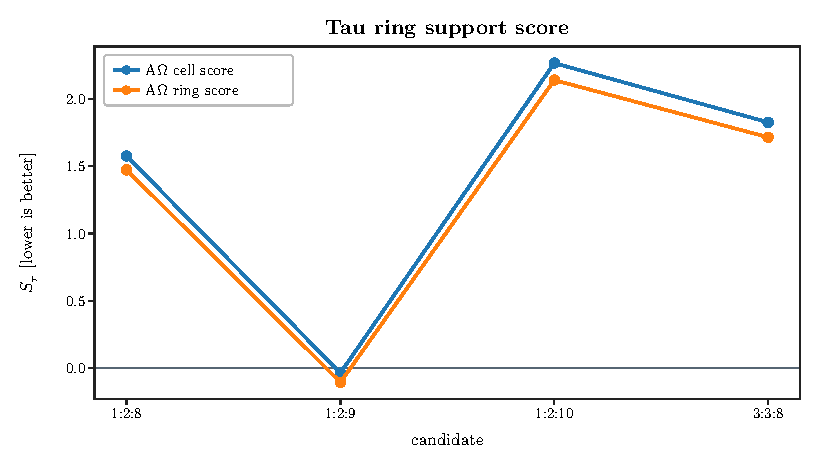
\includegraphics[width=0.92\linewidth,height=0.78\textheight,keepaspectratio]{figures/generated/tau-ring-support-score.pdf}
\caption{Tau ring support score. The ring diagnostic preserves $1:2:9_{\mathrm{yro}}$ / Dimonnanyro as the closest candidate.}
\label{fig:manual-tau-ring-score}
\end{figure}

\begin{figure}[H]
\centering
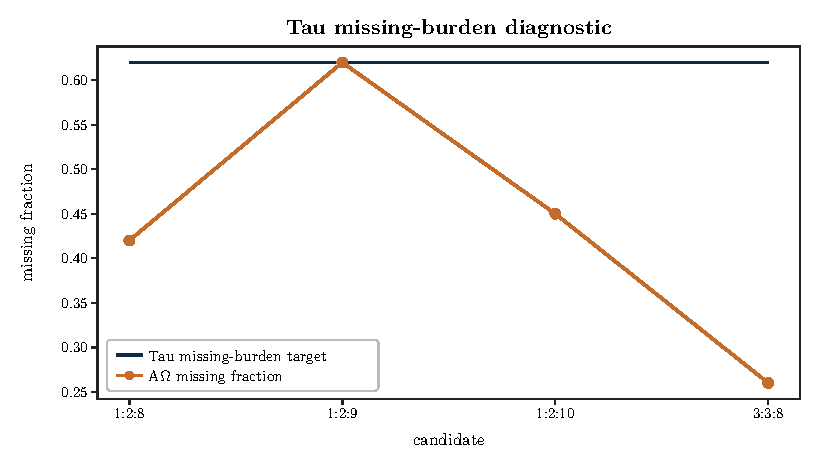
\includegraphics[width=0.92\linewidth,height=0.78\textheight,keepaspectratio]{figures/generated/tau-missing-burden-diagnostic.pdf}
\caption{Tau missing-burden diagnostic. The plot renders the exact missing-burden ratio $31/50$ as the presentation value $0.62$ for the $1:2:9_{\mathrm{yro}}$ / Dimonnanyro row.}
\label{fig:manual-tau-missing}
\end{figure}

\begin{figure}[H]
\centering
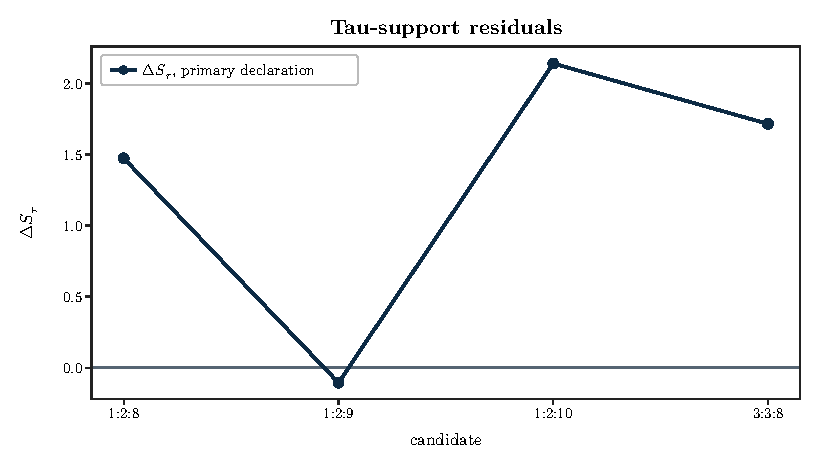
\includegraphics[width=0.92\linewidth,height=0.78\textheight,keepaspectratio]{figures/generated/tau-support-residuals.pdf}
\caption{Tau-support residuals against the declared support-score target.}
\label{fig:manual-tau-residuals}
\end{figure}

\begin{figure}[H]
\centering
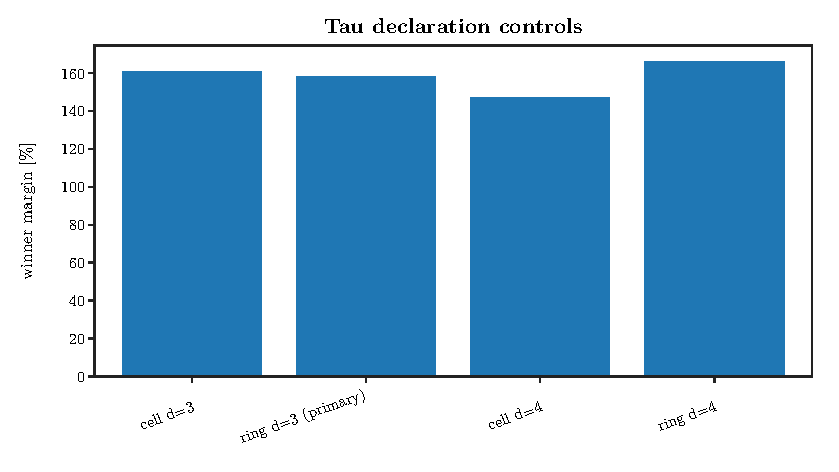
\includegraphics[width=0.92\linewidth,height=0.78\textheight,keepaspectratio]{figures/generated/tau-declaration-controls.pdf}
\caption{Tau declaration controls. Labels are declaration controls for the internal diagnostic lane.}
\label{fig:manual-tau-controls}
\end{figure}

\subsection{Milky Way / Gaia follow-up declaration}\label{manual:mw-gaia-followup}

The Sol bobbing record is recorded as a field dynamics diagnostic.

\[
B_{\mathrm{Sol}}|t=(\partial_TR_{\mathrm{Sol}}(t),\omega_{\mathrm{Sol}}|t).
\]

\[
\Phi^D_{\partial_TR,\mathrm{mov}}(t)=\Phi^D_{\mathrm{cross}}(t)-\Phi^D_{\mathrm{sweep}}(t)+\Phi^D_{\mathrm{shedding}}(t).
\]

A Gaia follow-up comparison is recorded after a benchmark target record is supplied.

\subsection{Orbital-retention field-dynamics fixture plan}\label{manual:orbital-retention-field-dynamics-fixture}

Data-support class: G2/G3 retention-first field-dynamics fixture. Its sequence is

\begin{align*}
 & \text{medium setup}\to\text{flip/fizz classification}\to\text{range-prioritized SADAR},\\ & \text{capacity seating}\to\text{orbital retention}\to\delta_3\text{ class tally},\\ & \text{optional }U\text{ diagnostic}.
\end{align*}

The fixture declares the flip classifier inside the manual/application layer:

\[
\operatorname{FlipClass}_{e,c,t}\in\{\mathrm{early\_coupling},\mathrm{fizz},\mathrm{pending},\mathrm{sheddic\_route}\}.
\]

The early-coupling indicator is

\[
G^{\mathrm{early}}_{e,c,t}=\mathbf{1}[\rho^D_{\omega,e,c,t}>0]\,\mathbf{1}[Q^D_{e,c,t}<Q_{\max}]\,C^{\theta}_{e,c,t}\,Z^{\mathrm{imp}}_{e,c,t}\,\mathbf{1}[\Delta A_{e,c,t}\ne0].
\]

When $G^{\mathrm{early}}_{e,c,t}>0$, the fixture records early coupling. Fizz records successor motion / background-continuation jitter. Pending records retained return carried over the current window. The class $\mathrm{sheddic\_route}$ records a flip carried through a declared sheddic path.

\paragraph{Orbital-retention input provenance gate.}
Before a scored orbital-retention run, the fixture records the data provenance of every field component used by the retained calculation. The input package records radial support rows; three-dimensional density fields; gas/stellar velocity fields; momentum fields; time-window/slosh fields; capacity rule; coupling family; sheddic-route declaration; and external value map when used. SPARC radial rows may populate the radial-support component. Three-dimensional density, velocity, current, and time-flow components are populated by their own declared source rows or proxy rows before scoring.

\begin{table}[H]
\centering
\caption{Orbital-retention input provenance gate.}
\label{tab:orbital-retention-input-provenance}
{\footnotesize
\begin{tabular}{>{\raggedright\arraybackslash}p{0.190\linewidth}>{\raggedright\arraybackslash}p{0.170\linewidth}>{\raggedright\arraybackslash}p{0.170\linewidth}>{\raggedright\arraybackslash}p{0.200\linewidth}>{\raggedright\arraybackslash}p{0.090\linewidth}}
\toprule
Field component & Source & Support status & Uncertainty status & Scored \\
\midrule
stellar radial support & SPARC radial model & SPARC-supported radial & radial source row & diagnostic \\
stars, full medium & 3D stellar density & external 3D & measured / proxy & if declared \\
gas, full medium & H I / H$\alpha$ / IFU field & external 3D & channel / velocity uncertainty & yes, if declared \\
core / background & model or survey & latent / proxy & proxy recorded & conditional \\
current-cycle family & A$\Omega$D range edges & declared proxy & declaration audit & internal \\
time-flow / slosh & kinematic window & external 3D / latent & cadence / window & conditional \\
external value map & quarantined map & declared proxy & frozen before scoring & external only \\
\bottomrule
\end{tabular}
}
\end{table}

\aodremark{A scored orbital-retention run records source, support status, uncertainty status, and whether each component is used for scoring before residuals are interpreted.}

\begin{table}[H]
\centering
\caption{Orbital-retention field-dynamics fixture spine.}
\label{tab:orbital-retention-fixture-spine}
{\footnotesize
\begin{tabular}{>{\raggedright\arraybackslash}p{0.080\linewidth}>{\raggedright\arraybackslash}p{0.340\linewidth}>{\raggedright\arraybackslash}p{0.420\linewidth}}
\toprule
No. & Sheet & Purpose \\
\midrule
00 & Declarations & Freeze declarations before scoring. \\
01 & Cell grid 3D & Declare the retained 3D cell grid. \\
02 & Input density fields & Declare star/gas/core/background/current density inputs and source/status records. \\
03 & Fractal range / max field support & Compute fractal range and maximum supported field count. \\
04 & Field regime & Declare gas/fluid/fizz regime. \\
05 & Chiral flip: early coupling vs fizz & Classify flips as early coupling, fizz, pending, or sheddic route. \\
06 & Range edge sets & Build range-prioritized coupling families. \\
07 & SADAR coupling / pressure / velocity & Compute SADAR coupling, pressure, and motion quantities. \\
08 & Capacity seating & Seat capacity by range and closure state. \\
09 & Hinge shift / partial coupling & Record hinge shift and partial coupling. \\
10 & Slosh / sheddic / pending & Record slosh, sheddic routing, and pending return. \\
11 & Orbital retention class & Classify orbital retention before projection. \\
12 & Delta3 retention tallies & Record exact $\delta_3$ retention tallies. \\
13 & U projection diagnostic & Optional square-speed diagnostic after retention scoring. \\
14 & Audit & Check declaration, retention, projection, and error layers. \\
\bottomrule
\end{tabular}
}
\end{table}

\aodremark{The SPARC square-speed lane is a G0 radial projection diagnostic. The orbital-retention fixture is the G2/G3 retention-first simulation path. Projection to $U$ follows retention, capacity seating, and $\delta_3$ tallies.}

\subsection{Completion requirements}\label{manual:field-dynamics-completion-requirements}

A SPARC score record is arithmetically complete when the data file, declaration constants, square-speed target, residuals, and score metrics are present. A Tau ring fixture is complete when the candidate set, scores, missing fraction, and precision note are present. Display speed is a presentation view only. The orbital-retention field-dynamics fixture is complete when it records medium setup, flip/fizz classification, range-prioritized SADAR, capacity seating, retention class, and $\delta_3$ tallies.
These are record-completeness conditions. Replay also requires the bound
producer and all operands; physical validation additionally requires the
source/uncertainty and independent-comparison evidence in
\secref{manual:prediction-test-registry}. Carried Tau scores and unsupported
declaration-control recipes remain carried records.

\subsection{Five-boundary hinge-saturation stepper and SPARC pooled D.E.C. ledger}\label{manual:field-dynamics:dec-run-tumble-stepper}

Declare the field-dynamics five-boundary stack

\[
B_{Q_4}\to B_{\mathrm{hinge}}\to B_{\mathrm{ring}}\to B_{\mathrm{pool}}\to B_{\mathrm{ext}}.
\]

Vectors \texttt{RC-041} and \texttt{RC-032} (\texttt{manual/data/boundary\_sadar/run\_tumble\_q4\_dec\_walk.csv} and \texttt{manual/data/boundary\_sadar/sparc\_pooled\_primary\_exact.csv}, verified by \texttt{python3 -B -m manual.engine} \texttt{--sector} \texttt{boundary\_sadar} and \texttt{aod-core} \texttt{--verify-vectors} \texttt{--check-zero-float}) reproduce all $21$ ticks of the $Q_4\to\mathbb{Z}^3$ run-tumble trace directly from the two-step hinge-saturation slide law ($\operatorname{adm}=0$ after two consecutive same-axis steps forces a tumble onto the next axis, closing back to $0000$ at $t=16$ with $Q_4-Q_3=h_4^2\ge0$) alongside the exact $209$-bin rational SPARC $U=V^2$ pooled score ($64.70291920$ \% display, zero free halo fitting).

\begin{figure}[H]
\centering
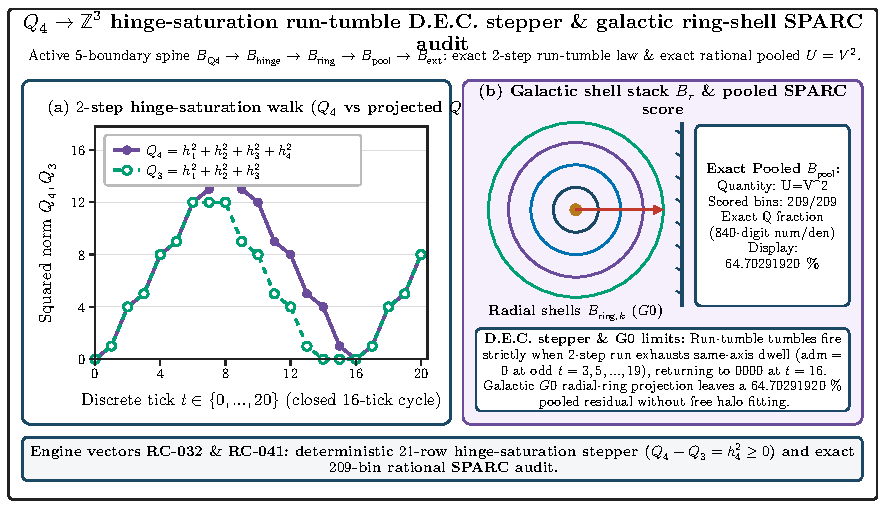
\includegraphics[width=0.92\linewidth,height=0.78\textheight,keepaspectratio]{figures/generated/field-dynamics-boundary-feynman.pdf}
\caption{Two-step hinge-saturation $Q_4\to\mathbb{Z}^3$ run-tumble D.E.C. trajectory ($Q_4$ versus projected $Q_3$) and concentric galactic radial-ring SPARC pooled audit (\texttt{run\_tumble\_q4\_dec\_walk.csv}, \texttt{sparc\_pooled\_primary\_exact.csv}).}
\label{fig:manual-field-dynamics-boundary-feynman}
\end{figure}

\begin{table}[H]
\centering
\caption{Two-step hinge-saturation $Q_4\to\mathbb{Z}^3$ run-tumble D.E.C. stepper checkpoints (\texttt{RC-041}; full $21$-tick trace in \texttt{run\_tumble\_q4\_dec\_walk.csv}).}
\label{tab:manual-field-dynamics-dec-spine}
{\footnotesize
\begin{tabular}{rllrlrrr}
\toprule
$t$ & Mode & Slot $(e,\sigma)$ & Dwell adm & $(h_1,h_2,h_3,h_4)$ & $Q_3$ & $Q_4$ & Octant \\
\midrule
0 & \texttt{init} & $-$ & 1 & $(0,0,0,0)$ & 0 & 0 & 0 \\
2 & \texttt{run} & $(e_1,+1)$ & 1 & $(2,0,0,0)$ & 4 & 4 & 0 \\
3 & \texttt{tumble} & $(e_2,+1)$ & 0 & $(2,1,0,0)$ & 5 & 5 & 0 \\
5 & \texttt{tumble} & $(e_3,-1)$ & 0 & $(2,2,-1,0)$ & 9 & 9 & 4 \\
7 & \texttt{tumble} & $(e_4,+1)$ & 0 & $(2,2,-2,1)$ & 12 & 13 & 4 \\
8 & \texttt{run} & $(e_4,+1)$ & 1 & $(2,2,-2,2)$ & 12 & 16 & 4 \\
16 & \texttt{run} & $(e_4,-1)$ & 1 & $(0,0,0,0)$ & 0 & 0 & 0 \\
20 & \texttt{run} & $(e_2,+1)$ & 1 & $(2,2,0,0)$ & 8 & 8 & 0 \\
\bottomrule
\end{tabular}
}
\end{table}
